\subsection{Cattura elettronica}

Nel processo di cattura elettronica nel \na{}
viene emesso solo il fotone del neon a \SI{1275}{keV} e non il positrone.
Vogliamo misurare il rapporto di decadimento della cattura elettronica.
Le uniche informazioni precise sui rate parziali le possiamo estrarre dai fotopicchi
perché sono le uniche parti dello spettro per cui abbiamo un modello (la gaussiana).

\subsubsection{Normalizzazione del rate}

L'ADC riesce a leggere solo una frazione degli eventi,
però è ragionevole supporre che la decimazione sia imparziale,
quindi per ottenere il rate parziale dallo spettro basta normalizzare
moltiplicando per il rate misurato dal contatore
e dividendo per il numero di eventi registrati dall'ADC.

\subsubsection{Fotopicchi}

\begin{figure}
	\centering
	INSERIRE DISEGNO
	\caption{\label{fig:fotopicchi}
	INSERIRE ciao}
\end{figure}

Usando due scintillatori possiamo ricavare il rate di nove fotopicchi diversi,
corrispodenti alle varie configurazioni con cui i fotoni possono interagire con i rivelatori
(vedi \autoref{fig:fotopicchi})\footnote{Non abbiamo considerato configurazioni con tre rivelatori per questa misura.}.
Indichiamo con $\beta$ i fotoni di annichilazione (\SI{511}{keV})
e con $\gamma$ i fotoni del neon (\SI{1275}{keV}).
Chiamiamo i rivelatori ``1'' e ``2''.
Cinque fotopicchi si ottengono dalle coincidenze a due:
\begin{description}
	\item[$\beta\beta$]
	Caso in cui entrambi i rivelatori vedono i fotoni di annichilazione contrapposti e li assorbono.
	Questo picco è presente solo se la sorgente è tra i due rivelatori.
	\item[$\gamma\beta$]
	Caso in cui il rivelatore 1 assorbe il fotone $\gamma$ e il 2 uno dei $\beta$.
	\item[$\beta\gamma$]
	Come $\gamma\beta$ ma con $\beta$ sul rivelatore 1 e $\gamma$ sul 2.
	\item[$(\beta,\gamma\beta)$]
	Il rivelatore 1 assorbe $\beta$ e il rivelatore 2 assorbe l'altro $\beta$ e $\gamma$.
	Come $\beta\beta$, questo segnale è presente solo se la sorgente si trova interposta tra i rivelatori.
	\item[$(\gamma\beta,\beta)$]
	Come il precedente ma con i rivelatori scambiati di ruolo.
\end{description}
Gli altri quattro fotopicchi si ottengono triggerando su uno scintillatore alla volta:
per ogni scintillatore di ottiene un picco $\beta$ e un $\gamma$,
distinguiamo i rivelatori con un pedice: $\beta_1$, $\gamma_1$, $\beta_2$, $\gamma_2$.

\subsubsection{Equazioni dei rate}

Per ogni fotopicco misuriamo il rate.
Scrivendo i rate in funzione delle efficienze e accettanze dei rivelatori
e in funzione del rate di $\beta$ e del rate di $\gamma$
(diversi perché c'è la cattura elettronica)
otteniamo un sistema di equazioni da cui dobbiamo ricavare i rate.
Poiché in generale l'accettanza e l'efficienza non sono fattorizzate le teniamo combinate.
Usiamo le variabili:
\newcommand*\tot{^\text{tot}}
\newcommand*\R{r}
\newcommand*\Rtot{\mathcal{R}}
\begin{description}
	\item[$\R$:]
	Rate $\beta$.
	\item[$\Rtot$:]
	Rate $\gamma$, ovvero $r$ più il rate di cattura elettronica.
	\item[$p_{\beta1}$, $p_{\beta2}$, $p_{\gamma1}$, $p_{\gamma2}$:]
	Probabilità di assorbimento per i vari fotoni/rivelatori.
	\item[$p_{\beta12}$:]
	Probabilità di assorbimento in coincidenza dei due fotoni $\beta$.
	\item[$p_{\beta1}^\text{tot}$, $p_{\beta2}^\text{tot}$, $p_{\gamma1}^\text{tot}$, $p_{\gamma2}^\text{tot}$:]
	Probabilità di rivelazione totali per i vari fotoni/rivelatori,
	cioè in pratica rispetto alle variabili senza apice è incluso il caso in cui il fotone fa Compton.
	\item[$p_{\beta12}^\text{tot}$:]
	Probabilità di rivelazione totale per i fotoni in coincidenza
	\emph{con l'esclusione del caso in cui fanno entrambi Compton}.
	\item[$R_{\beta1}$, $R_{\beta2}$, $R_{\gamma1}$, $R_{\gamma2}$, $R_{\beta\beta}$, $R_{\gamma\beta}$, $R_{\beta\gamma}$, $R_{\beta,\gamma\beta}$, $R_{\gamma\beta,\beta}$:]
	Rate dei vari fotopicchi.
\end{description}
Le equazioni sono
\begin{align}
	R_{\beta\beta} \label{eq:betabeta}
	&= \R p_{\beta12} (1 - p_{\gamma1}\tot - p_{\gamma2}\tot) \\
	R_{\gamma\beta} \label{eq:gammabeta}
	&= 2\R p_{\beta2} p_{\gamma1} - \R p_{\beta12}\tot p_{\gamma1} \\
	R_{\beta\gamma} \label{eq:betagamma}
	&= 2\R p_{\beta1} p_{\gamma2} - \R p_{\beta12}\tot p_{\gamma2} \\
	R_{\beta,\gamma\beta} \label{eq:betagammabeta}
	&= \R p_{\beta12} p_{\gamma2} \\
	R_{\gamma\beta,\beta} \label{eq:gammabetabeta}
	&= \R p_{\beta12} p_{\gamma1} \\
	R_{\beta1}
	&= 2\R p_{\beta1} (1 - p_{\gamma1}\tot) \\
	R_{\gamma1} \label{eq:gamma1}
	&= p_{\gamma1}(\Rtot - 2 \R p_{\beta1}\tot) \\
	R_{\beta1}
	&= 2\R p_{\beta2} (1 - p_{\gamma2}\tot) \\
	R_{\gamma2} \label{eq:gamma2}
	&= p_{\gamma2} (\Rtot  - 2 \R p_{\beta2}\tot).
\end{align}
Nel caso in cui la sorgente non sia interposta tra i rivelatori
bisogna eliminare le equazioni \eqref{eq:betabeta}, \eqref{eq:betagammabeta}, \eqref{eq:gammabetabeta}
e porre $p_{\beta12}\tot = 0$ in \eqref{eq:gammabeta} e \eqref{eq:betagamma}.

Notiamo che $\Rtot$ compare solo nelle equazioni \eqref{eq:gamma1} e \eqref{eq:gamma2}.
Notiamo anche che $\R$ compare solo a moltiplicare le variabili
$p_{\beta1}$, $p_{\beta2}$, $p_{\beta12}$, $p_{\beta1}\tot$, $p_{\beta2}\tot$, $p_{\beta12}\tot$
e che, viceversa, queste compaiono solo a moltiplicare $\R$,
cioè questo insieme di 7 variabili è degenere e va ridotto alle 6 variabili
$\R p_{\beta1}$, $\R p_{\beta2}$, $\R p_{\beta12}$, $\R p_{\beta1}\tot$, $\R p_{\beta2}\tot$, $\R p_{\beta12}\tot$,
quindi non si può ricavare $\R$.
Il sistema è a 9 equazioni con 11 incognite,
quindi bisogna necessariamente fare approssimazioni o aggiungere equazioni anche per ricavare $\Rtot$.

\subsubsection{Informazioni esterne}

Per aggiungere equazioni e ricavare $\Rtot$
prendiamo valori tabulati di $p_{\dots} / p_{\dots}\tot$ da [KNOLL].
[KNOLL] fornisce il rapporto per scintillatori da $\SI{2}{''}\times\SI2{''}$ a \SI{10}{cm},
quindi quando usiamo distanze diverse aggiungiamo un'incertezza stimata grossolanamente ai rapporti tabulati.
I rapporti sono
$p_\beta / p_\beta\tot = \SI{50(2)}\%$ e
$p_\gamma / p_\gamma\tot = \SI{22(2)}\%$.
Ricaviamo $p_{\beta12} / p_{\beta12}\tot$ facendo l'approssimazione che valga
$p_{\beta12}\propto p_{\beta1}p_{\beta2}$ cioè che le probabilità si fattorizzino.
Allora
\marginpar{Non si capisce una fava.}
\begin{align*}
	\frac{p_{\beta12}\tot}{p_{\beta12}}
	&= \frac
	{p_{\beta1}p_{\beta2} + (p_{\beta1}\tot - p_{\beta1}) p_{\beta2} + p_{\beta1} (p_{\beta2}\tot - p_{\beta2})}
	{p_{\beta1}p_{\beta2}} = \\
	&= \frac{p_{\beta1}\tot}{p_{\beta1}} + \frac{p_{\beta2}\tot}{p_{\beta2}} - 1.
\end{align*}

\subsubsection{Fattorizzazione delle probabilità}

I rapporti $p_{\dots} / p_{\dots}\tot$ non sono sufficienti per ricavare $\R$.
Per rompere la degenerazione bisogna scrivere le probabilità in termini di accettanze e efficienze.
Nel modello più semplice le probababilità sono fattorizzate in accettanza$\times$efficienza
e $p_{\beta12}$ è fattorizzato in termini dei due rivelatori.
Chiamiamo $A_1$ e $A_2$ le accettanze dei due rivelatori,
$A_{12}$ l'accettanza per i fotoni di annichilazione in coincidenza,
$P_1$ e $P_2$ le efficienze.
Allora
\begin{align*}
	p_{\beta1}
	&= A_1 P_1, \\
	p_{\beta2}
	&= A_2 P_2, \\
	p_{\beta12}
	&= A_{12} P_1 P_2.
\end{align*}
Se dalle equazioni ricaviamo $\R p_{\beta1}$, $\R p_{\beta2}$ e $\R p_{\beta12}$ abbiamo che
\begin{align*}
	\frac {\R p_{\beta1} \cdot \R p_{\beta2}} {\R p_{\beta12}}
	&= \R \frac{A_1 A_2}{A_{12}},
\end{align*}
quindi possiamo ricavare $r$ misurando le accettanze.

\subsubsection{Misura}

\begin{figure}
	\hspace{-0.2\textwidth}
	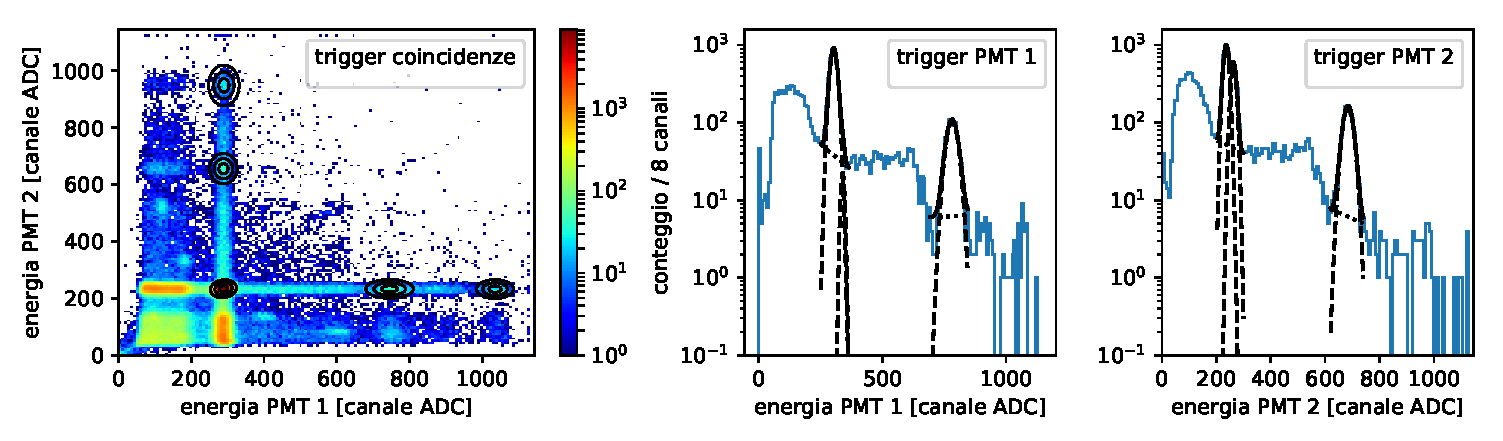
\includegraphics[width=1.4\textwidth]{immagini/ec}
	\caption{\label{fig:ec}
	ciao}
\end{figure}

\paragraph{Apparato}

Poniamo i due scintillatori allineati uno davanti all'altro usando la guida metallica,
con le facce a distanza \SI{9.0 \pm 0.1}{cm}.
La guida permette di farli scorrere quindi controlliamo che siano allineati
facendo appoggiare le facce e poi allontanandoli.
Attacchiamo un righello da uno scintillatore all'altro per posizionare la sorgente al centro.
Attacchiamo la sorgente a un supporto che possiamo far scorrere fino ad appoggiarlo ai rivelatori
per controllare che sia allineata al centro.
Controlliamo gli allineamenti con foto da varie angolazioni.

\paragraph{Accettanze}

L'accettanza non è ben definita perché gli scintillatori non sono tronchi di corone sferiche.
Per tenerne conto calcoliamo l'accettanza dall'area sottesa dalla circonferenza dello scintillatore
a 1/3 e 2/3 della profondità, prendiamo la media delle due come accettanza e la differenza come incertezza.
Poiché la sorgente è ben allineata, l'accettanza per le coincidenze a 2 è la stessa.
Risulta $A_1 = A_2 = A_{12} = \num{0.028(12)}$.

\paragraph{Fit dei picchi}


